\documentclass[11pt]{article}
\usepackage[margin=1in]{geometry}
\usepackage{graphicx}
\usepackage{microtype}
\usepackage{verbatim}
\usepackage{amsmath}
\usepackage{nicefrac}
\usepackage[colorlinks=false, pdfborder={0 0 0}]{hyperref}
\begin{document}
\title{Rudder Controller \& Wiper Controller\\Embedded System Design, Lab 2}
\date{September 25, 2015}
\author{Ben Lorenzetti}
\maketitle
\tableofcontents

\clearpage

\section{Objectives and Problem Description}

The primary objective of this lab was learning to interface with two new types of peripherals: a servo motor and potentiometers.
Several new functions in PBASIC are introduced for these types of actuators and transducers.

\subsection{Rudder Controller}

Control the angular position of a tiny ship's rudder (i.e. the horn of your servo)
based on the input from a steering wheel (i.e. your potentiometer).
The full range of motion of the ship's rudder should be $45^{o}<\theta<135^{o}$
and it should be controlled linearly by the full range of the potentiometer.

\subsection{Wiper Controller}

Instead of controlling angular position, as was done for the rudder controller,
use the potentiometer to control the angular velocity of the servo.
The servo represents a single windshield wiper, and should rotate continuously
between $15^{o}$ and $160^{o}$. The full range of the potentiometer should
be used to linearly control the wiper speed from 0 degrees/sec up to the
maximum speed.

\section{Procedure}
\subsection{Assignment: Ch. 4 Servo Motor}

To prepare for this lab, we were instructed to read chapters 4 and 5 in the Parallax What's a Microcontroller book and complete the example activities.

The parallax servo motor has three connectiong: power, ground, and signal.
The signal (white) connection is used to control the angular position of
the horn, from $0^{o}$ to $180^{o}$.
The servo expects a square wave control signal,
where the period is approximately 20 ms
and the width of the high pulse carries angular displacement information.

\begin{figure}[h!]
\centering
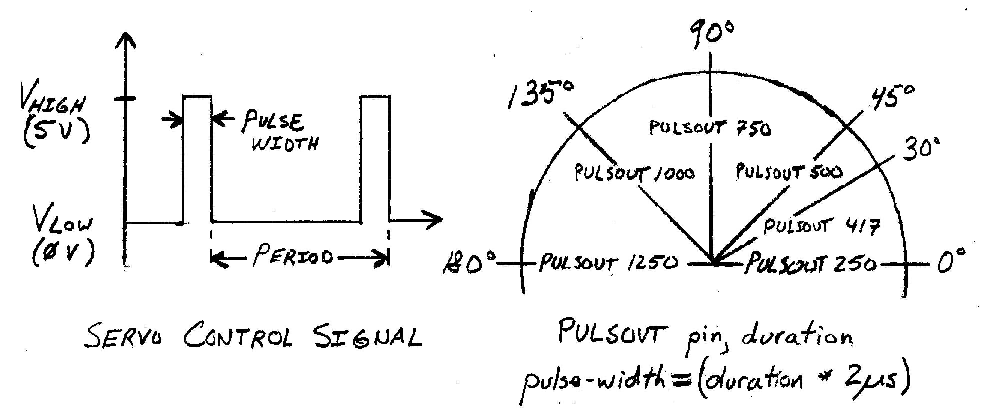
\includegraphics[width=0.8\textwidth]{pulse-width-vs-angular-displacement.pdf}
\caption{Servo Control Signal Timing}
\label{pulse-width-vs-angular-displacement}
\end{figure}

The formula relating pulse width and angular displacement is
\begin{equation}
t_{p-width}(\theta)=\left\{\begin{array}{c c}
\frac{500\mu s}{45^{o}}\theta+500\mu s	&	10^{o}<\theta<170^{o}\\
0\mu s	&	\textrm{servo off}	\\
\end{array}\right.
\label{pulse-width-eq}
\end{equation}

The function for doing pulse width modulation in PBASIC is
\texttt{PULSOUT pin, duration}, where \texttt{pin} is the
I/O port number and \texttt{duration} is the length of time high.
Of course, since this Stamp and PBASIC, the board isn't quite
fast enough so \texttt{duration} is in units of $2\mu s$ and
you have to complete the pulse width modulation yourself by
\texttt{PAUSE}ing for 20 ms, or however long the period should
be approximately.

To avoid dealing with PBASICs strange limitations,
we can rewrite equation \ref{pulse-width-eq} as
\begin{equation}
\textrm{duration}=\frac{50}{9}*\theta+250, \quad 10^{o}<\theta<170^{o}
\label{duration-eq}
\end{equation}

Chapter 4 also provided two more expressions in PBASIC that are helpful with servo motors:
\begin{verbatim}
i VAR Word
FOR i = 0 TO 150
	...
LOOP
}
\end{verbatim}
and
\texttt{duration = duration MIN 350 MAX 1150}.

\subsection{Assignment: Ch.5 Potentiometers}

Not surprisingly, the Basic Stamp is too primative to have an analog-to-digital converter,
so you can only measure analog inputs with a function called \texttt{RCTIME},
and then only if you construct an RC decay circuit--and again only if the input
signal is stable for a long enough charging time and can source enough current.

The function prototype is \texttt{RCTIME pin, state, duration},
where \texttt{pin} is the I/O pin number (0-15), \texttt{state} is the
expected charged status of the pin (0 or 1), and \texttt{duration} is
a variable to store the decay time--in units of $2\mu s$.
The decay time is taken when the voltage on \texttt{pin} falls below
$1.4V$, if the original charge \texttt{state} was 1.

\begin{figure}[h!]
\centering
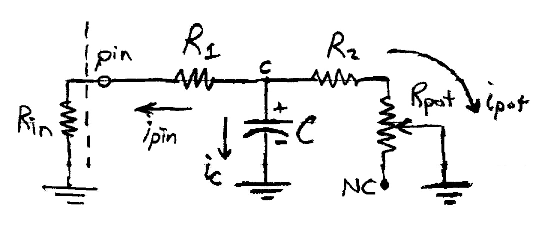
\includegraphics[width=0.5\textwidth]{pot-input-circuit.pdf}
\caption{Input Circuit for Reading a Potentiometer with \texttt{RCTIME}}
\label{pot-input-circuit}
\end{figure}

An input source that is well suited to \texttt{RCTIME} is a rotary
potentiometer. A circuit combining a potentiometer and capacitor is shown
if \hyperref[pot-input-circuit]{figure \ref{pot-input-circuit}}.

If we assume infinite input resistance once \texttt{RCTIME} switches
the pin direction to input, then $i_{pin}=0$ and $V_{in}=V_{c}$.
Taking Kirchoff's Current Law at node c allows us to solve for input
voltage as a function of time and initial condition across C.
\begin{equation*}
i_{pin}+i_{c}+i_{pot}=0
\end{equation*}
\begin{equation*}
0+C\frac{dV_{in}}{dt}+\frac{V_{in}}{R_{2}+R_{pot}}=0
\end{equation*}
\begin{equation*}
\frac{-V_{in}}{R_{2}+R_{pot}}=C\frac{dV_{in}}{dt}
\end{equation*}
\begin{equation*}
\frac{-1}{C(R_{2}+R_{pot})}*dt=\frac{1}{V_{in}}*dV_{in}
\end{equation*}
\begin{equation*}
\frac{-t}{C(R_{2}+R_{pot})}+A=ln(V_{in})
\end{equation*}
\begin{equation*}
e^{ln(V_{in})}=e^{\frac{-t}{C(R_{2}+R_{pot})}}
\end{equation*}
\begin{equation*}
V_{in}=e^{A}*e^{\nicefrac{-t}{C(R_{2}+R_{pot})}}
\end{equation*}
\begin{equation}
V_{in}(t)=V_{0}e^{-t/\tau} \quad \quad \tau=(R_{2}+R_{pot})C
\label{rc-decay-eq}
\end{equation}

Using equation \ref{rc-decay-eq}, the decay time required to discharge
from $V_{HIGH}$ to $V_{LOW}$ is
\begin{equation*}
V_{LOW}=V_{HIGH}e^{\nicefrac{-t_{discharge}}{\tau}}
\end{equation*}
\begin{equation*}
t_{discharge}=\tau*ln\left(\frac{V_{HIGH}}{V_{LOW}}\right)
\end{equation*}
For $V_{HIGH}=5V$, $V_{LOW}=1.4V$, $C=0.1\mu F$, this evaluates to
\begin{equation}
t_{discharge}=\left[\frac{6.365}{10^{2}}*\frac{2\mu s}{\Omega}\right]*(R_{2}+R_{pot})
\label{t-discharge-eq}
\end{equation}

A $10k\Omega$ potentiometer with $R_{2}=10k\Omega$, leads to input
domain $10k\Omega<R_{2}+R_{pot}<20k\Omega$ and output range
$636.48*2\mu s<t_{discharge}<1272.97*2\mu s$. When we consider
that the PBASIC Stamp board only has an integer resolution of
$2 \mu s$, then the expected result from a call to
\mbox{\texttt{RCTIME, pin, 1, duration}} is in the set
\begin{equation*}
\textrm{\texttt{duration}}=\{637, 638, 639,...1272, 1273\}
\end{equation*}
when used with a 0.1 $\mu F$ capacitor.

Actual testing showed with the circuit shown in
\hyperref[rudder-circuit]{figure \ref{rudder-circuit}}
showed an experimental range of
\begin{equation}
\textrm{\texttt{duration}}=\{619, 620, 621,...1288, 1289\}
\label{discharge-time-domain}
\end{equation}

\subsection{Rudder Controller}

\begin{figure}[h!]
\centering
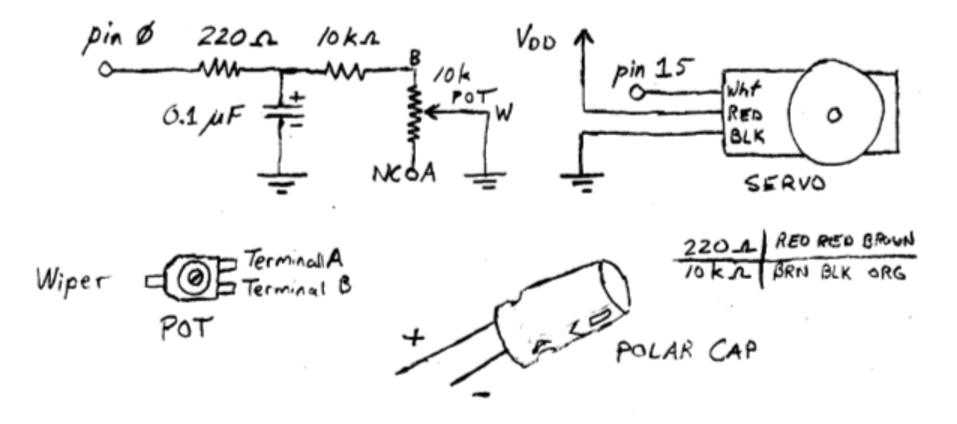
\includegraphics[width=.7\textwidth]{rudder-circuit.pdf}
\caption{Rudder Controller and Wiper Controller Circuit}
\label{rudder-circuit}
\end{figure}

The circuit contructed for the rudder controller is shown in figure
\ref{rudder-circuit}. In the potentiometer input circuit, a 220 $\Omega$
resistor is used to prevent a current inrush greater than the maximum
I/O pin current for the microcontroller.
\begin{equation*}
R_{limiter(MIN)}=\frac{V_{CC}-V_{SS}}{I_{I/O(MAX)}}=\frac{5V}{25mA}=200\Omega
\end{equation*}

The transient discharge of this potentiometer circuit was solved in
equation \ref{rc-decay-eq}, assuming that the charged voltage was nearly 5V.
To ensure that the potentiometer's parallel path to ground does not significantly
affect the charging time or the charging potential, resistor $R_{2}$ was
selected to be 10 $k\Omega$ such that $R_{2}+R_{pot}>>R_{1}$ for all values
of $R_{pot}$. With this assumption, charging current through $R_{pot}$
can be neglected and the charging time is approximately
\begin{equation*}
\tau_{charge}=220\Omega*0.1\mu F=0.022 ms
\end{equation*}
Based on $\tau_{charge}$, a charging \texttt{PAUSE} of 1 ms is more than adequate.

From theory (\hyperref[t-discharge-eq]{equation \ref{t-discharge-eq}})
and testing (\hyperref[discharge-time-domain]{set \ref{discharge-time-domain}}),
the domain of input discharge time values is 619--1289.
The output range should drive the servo between $45^{o}$--$135^{o}$.
Using \hyperref[duration-eq]{equation \ref{duration-eq}}, the output
range should be 500--1000. The mapping should be linear:
\begin{equation*}
y_{2}-y_{1}=m(x_{2}-x_{1})
\end{equation*}

\begin{equation*}
1000-500=m(1289-619)
\end{equation*}

\begin{equation*}
m=0.746=\frac{191}{256}
\end{equation*}

\begin{equation*}
y_{2}=0.746(x_{2}-619)+500
\end{equation*}

The microcontroller cannot do floating point arithmetic, but it does
have a fractional (middle) multiplication operator that allows you
to multiply by fractions of 256. Thus the final mapping equation is
\begin{equation}
t_{p-width}=\frac{191}{256}(t_{discharge-time}-619)+500
\end{equation}
where both times are in units of $2\mu s$. This is implemented:

\begin{center}
\mbox{\texttt{pulse\_width = ((discharge\_time - 619) */ 191) + 500}}
\end{center}

Once the potentiometer circuit's discharge time has been mapped
to a pulse width, all that remains is to output the pulse and loop
indefinitely with an appropriate delay period to complete the pulse-
width modulation and input monitoring. The flowchart for the implentation
is shown in \hyperref[rudder-flowchart]{figure \ref{rudder-flowchart}}.

\begin{figure}[ht]
\centering
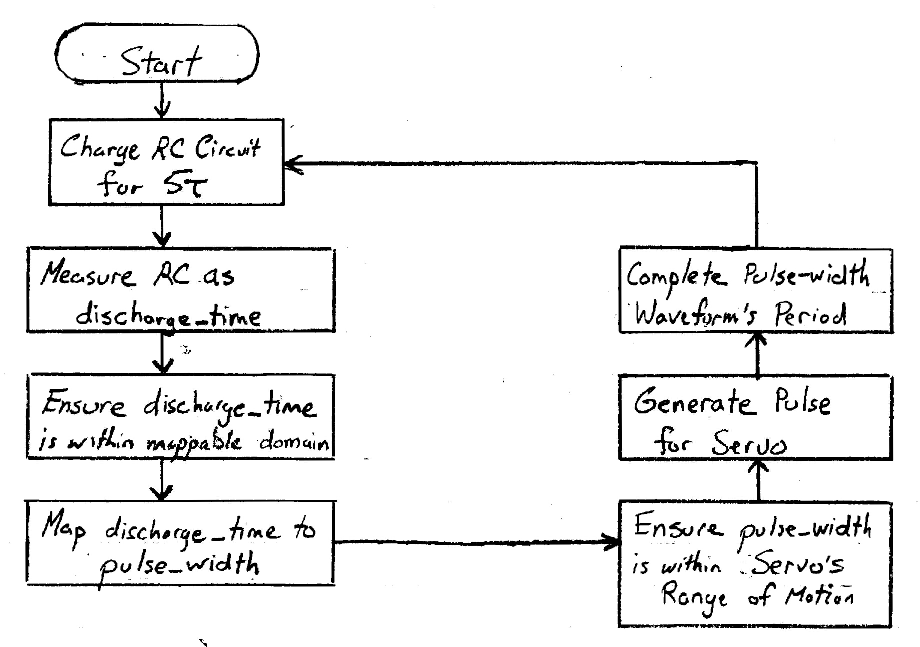
\includegraphics[width=0.65\textwidth]{rudder-flowchart.pdf}
\caption{Rudder Controller Implementation Flowchart}
\label{rudder-flowchart}
\end{figure}

\subsection{Wiper Controller}

The wiper controller used the same circuit as the rudder controller
(\hyperref[rudder-circuit]{figure \ref{rudder-circuit}}); the only
difference between the two is the implementation. The rudder controls
angular position, while the wiper implementation controls angular speed.

The maximum frequency at which the pulse width, and thus angular position,
can be changed is the inverse of the pulse width period.
\begin{equation*}
f_{max}=\frac{1}{T}=\frac{1}{20ms}=50 Hz
\end{equation*}

At this frequency (or a integer fraction of this frequency),
angular velocity can be controled by varying the magnitude
of change in pulse width per period.
\begin{equation}
\omega\propto\frac{\Delta(\textrm{pulse width})}{T}
\end{equation}

The maximum value for $\Delta$pulse\_width comes from the full range
of motion, which is specified for this project as $15^{o}<\theta<160^{o}$.
From \hyperref[duration-eq]{equation \ref{duration-eq}},
this corresponds to \mbox{\texttt{333 < duration < 1139}}.
So the maximum potential swing per period is
\begin{equation*}
1139-333=806*[2\mu s]
\end{equation*}

For smoothness, we will reduce the maximum swing per period
by a factor of 16 (somewhate arbitrarily), leaving us with 50 possible speeds.
Now, like was done for the rudder controller, the discharge\_time domain of 619--1289
needs to be mapped linearly to 50 speeds, starting at speed 0.
\begin{equation*}
50-0=m(1289-619)
\end{equation*}

\begin{equation*}
m=0.0746\approx\frac{19}{256}
\end{equation*}

\begin{equation}
\Delta\textrm{pulse\_width}_{(\textrm{per period})}=\frac{19}{256}(t_{\textrm{discharge}}-619)
\end{equation}
where again the pulse width, discharge time, and 619 constant are in units of 2 $\mu s$.

We have the the pulse width interval the wiper's range of motion,
we have a function for potentiometer input from the rudder project,
we have a mapping between the potentiometer discharge time and rate of change in pulse width;
all that is needed is an implementation. The implementation flowchart
is more complicated than the rudder controller because the wiper has to
continuously rotate between two extremes and change directions, in addition
to monitoring the pot. and varying speed. How this is done is shown in the
implementation flowchart in \hyperref[wiper-flowchart]{figure \ref{wiper-flowchart}}.

\begin{figure}[ht]
\centering
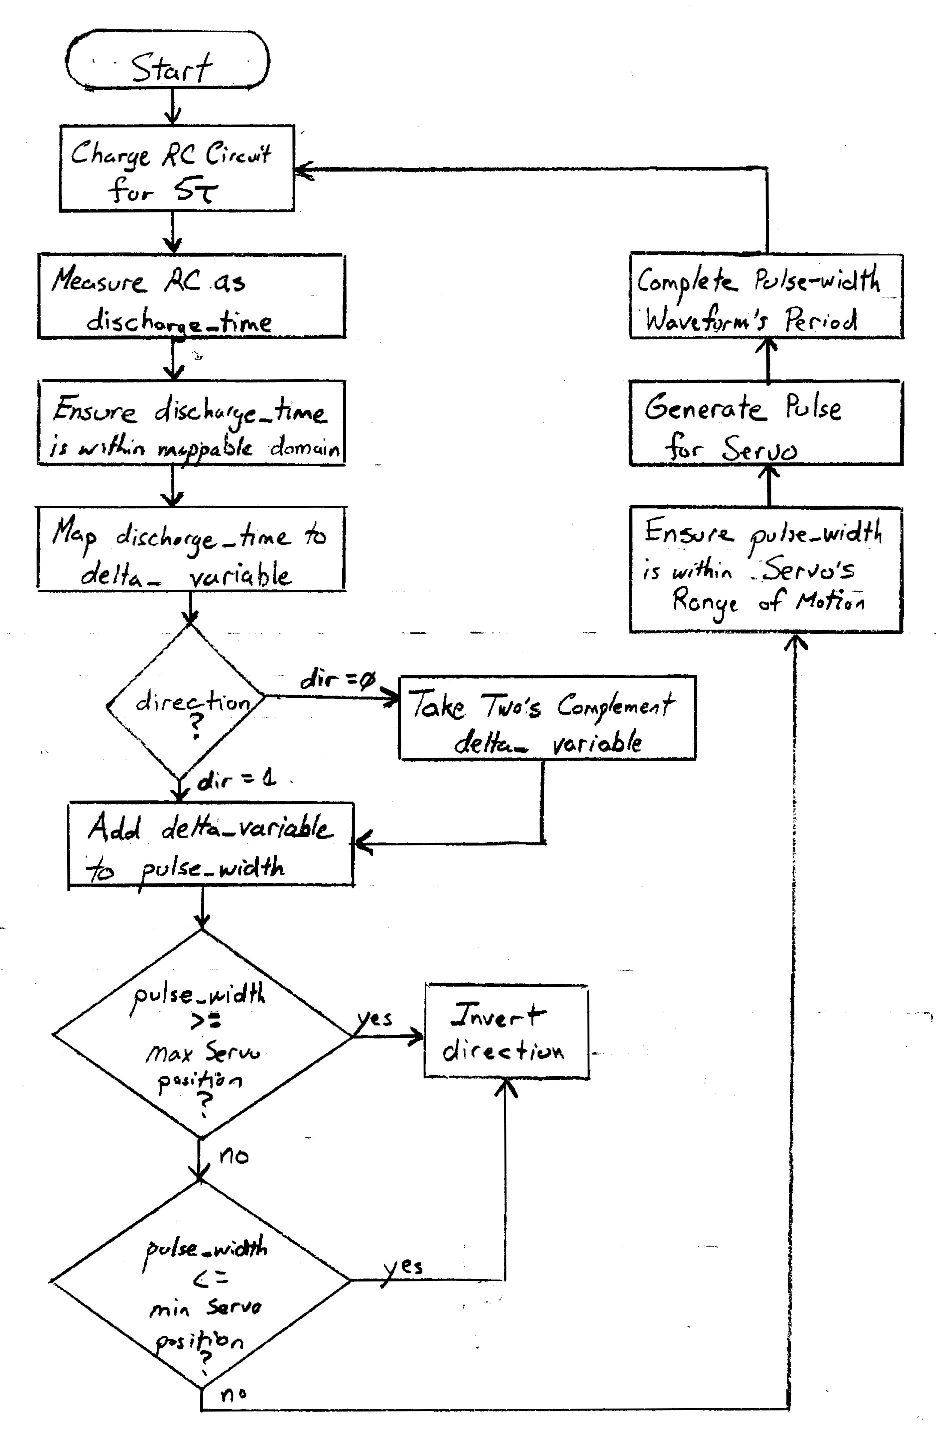
\includegraphics[width=0.65\textwidth]{wiper-flowchart.pdf}
\caption{Wiper Controller Flowchart}
\label{wiper-flowchart}
\end{figure}

\section{Expected Results}

I expected both circuits to behave according to the problem statements.

\section{Experiment and Design Revisions}

\subsection{Rudder Controller}

When I first built this project's implementation, the controller worked
for 90\% of the potentiometer's input range. However, when the discharge
time was on the lower range of its possible values, the rudder would
suddenly shift from near $45^{o}$ to the $135^{o}$ position.
After adding a \texttt{DEBUG} statement, I saw the following transition
occuring:
\begin{verbatim}
discharge_time = 622, pulse_width = 502
discharge_time = 621, pulse_width = 501
discharge_time = 620, pulse_width = 500
discharge_time = 619, pulse_width = 500
discharge_time = 618, pulse_width = 1000
\end{verbatim}

What was occuring was that the \texttt{discharge\_time} from the RC circuit
was coming back slightly lower than the minimum value I was expecting.
Thus the subraction \mbox{\texttt{(discharge\_time - MAPPING\_X1)}} resulted
in a negative number, except the variable was not declared as signed so
the result of the two's-complement arithmetic was the maximum possible
value for the 16-bit Word. Later in the code is the function
\mbox{\texttt{MAX 1000}}, so that is where the 1000 is coming from.

The fix for this bug was very simple, simply treating the
\texttt{discharge\_time} variable with \mbox{\texttt{MIN MAPPING\_X1}}
prior to calculating the \texttt{pulse\_width}.

\subsection{Wiper Controller}

When I first implemented this circuit the program worked but the servo
was extremely jerky. At first I thought this meant my speeds were too
high, but it turned out it was only due to a \texttt{DEBUG} statement
in the loop that was throwing off the pulse width timing.

Removal of the \texttt{DEBUG} statement fixed the error.

Another bug was that at the higher speeds the servo did not have
time to swing the full range of motion before a new command was
recieved in the opposite direction. To fix this, I added a second
pulse width in every iteration of the loop to reduce the maximum
speed by half.

\section{Observations}

Both circuits eventually worked as expected, and photos of the working boards are shown in
\hyperref[rudder-controller]{figure \ref{rudder-controller}}
and \hyperref[wiper-controller]{figure \ref{wiper-controller}}.

\begin{figure}
\centering
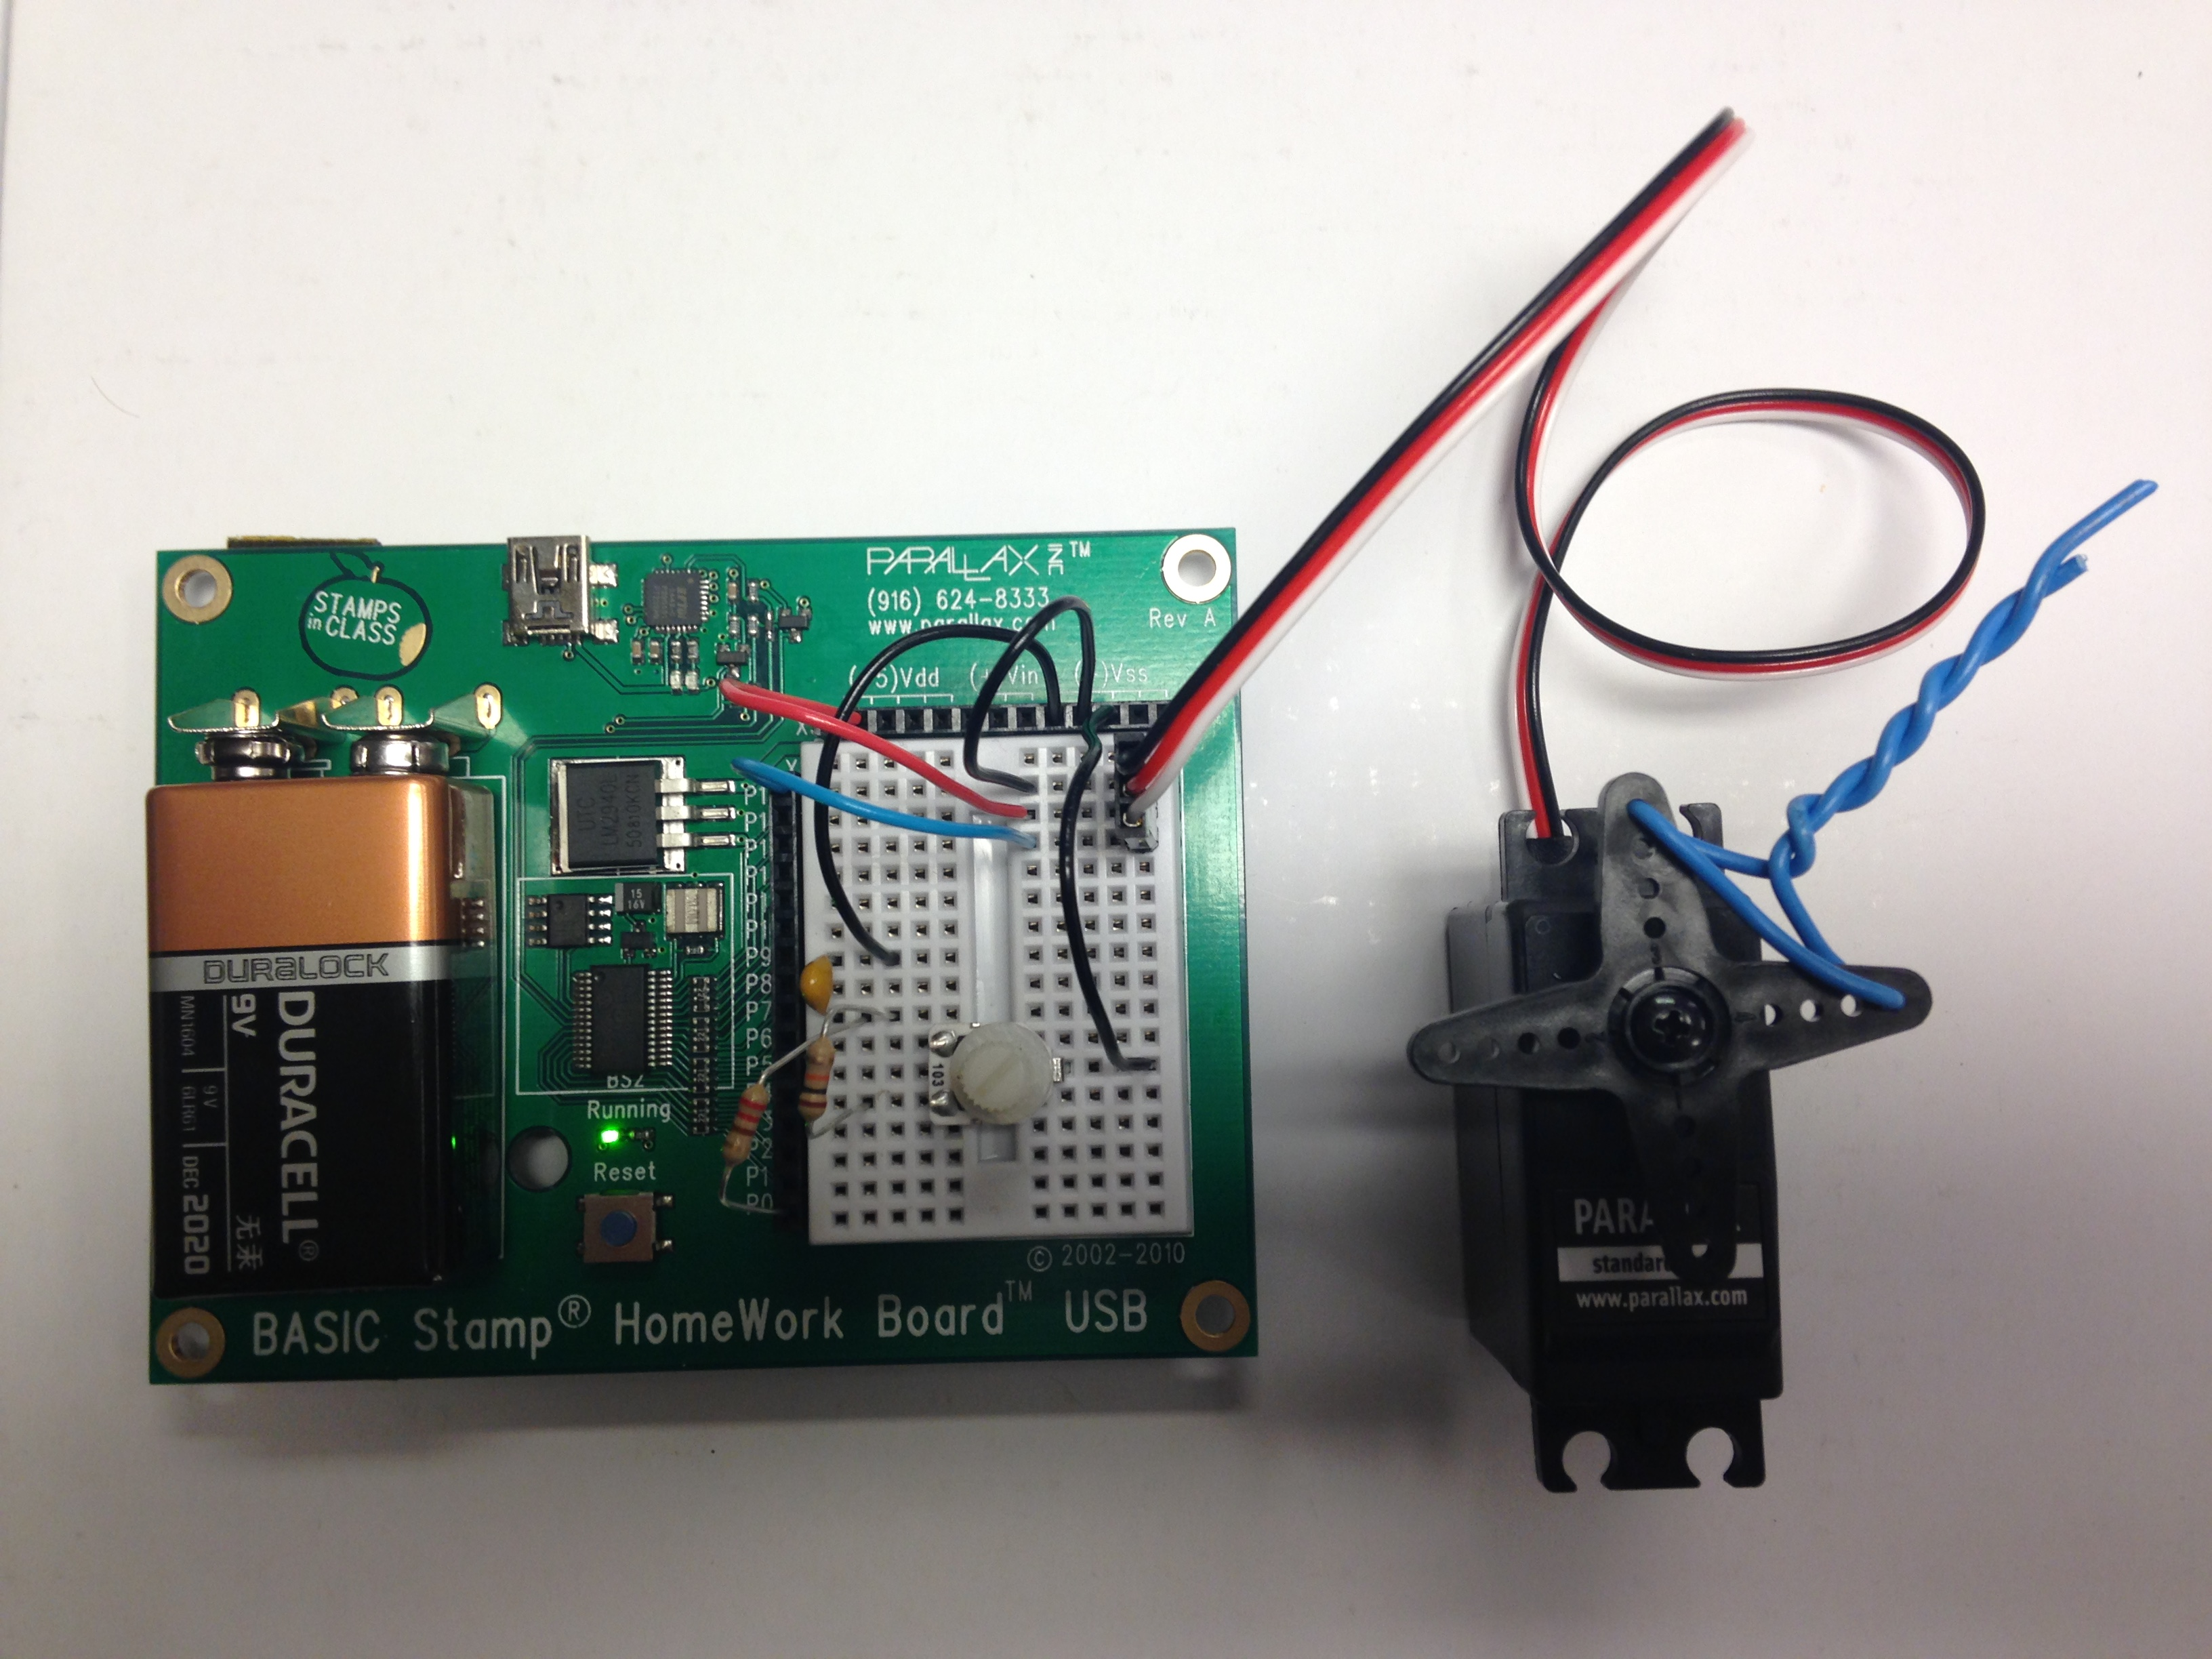
\includegraphics[width=0.6\textwidth]{rudder-controller.jpg}
\caption{Rudder Position Controller Board}
\label{rudder-controller}
\end{figure}

\begin{figure}
\centering
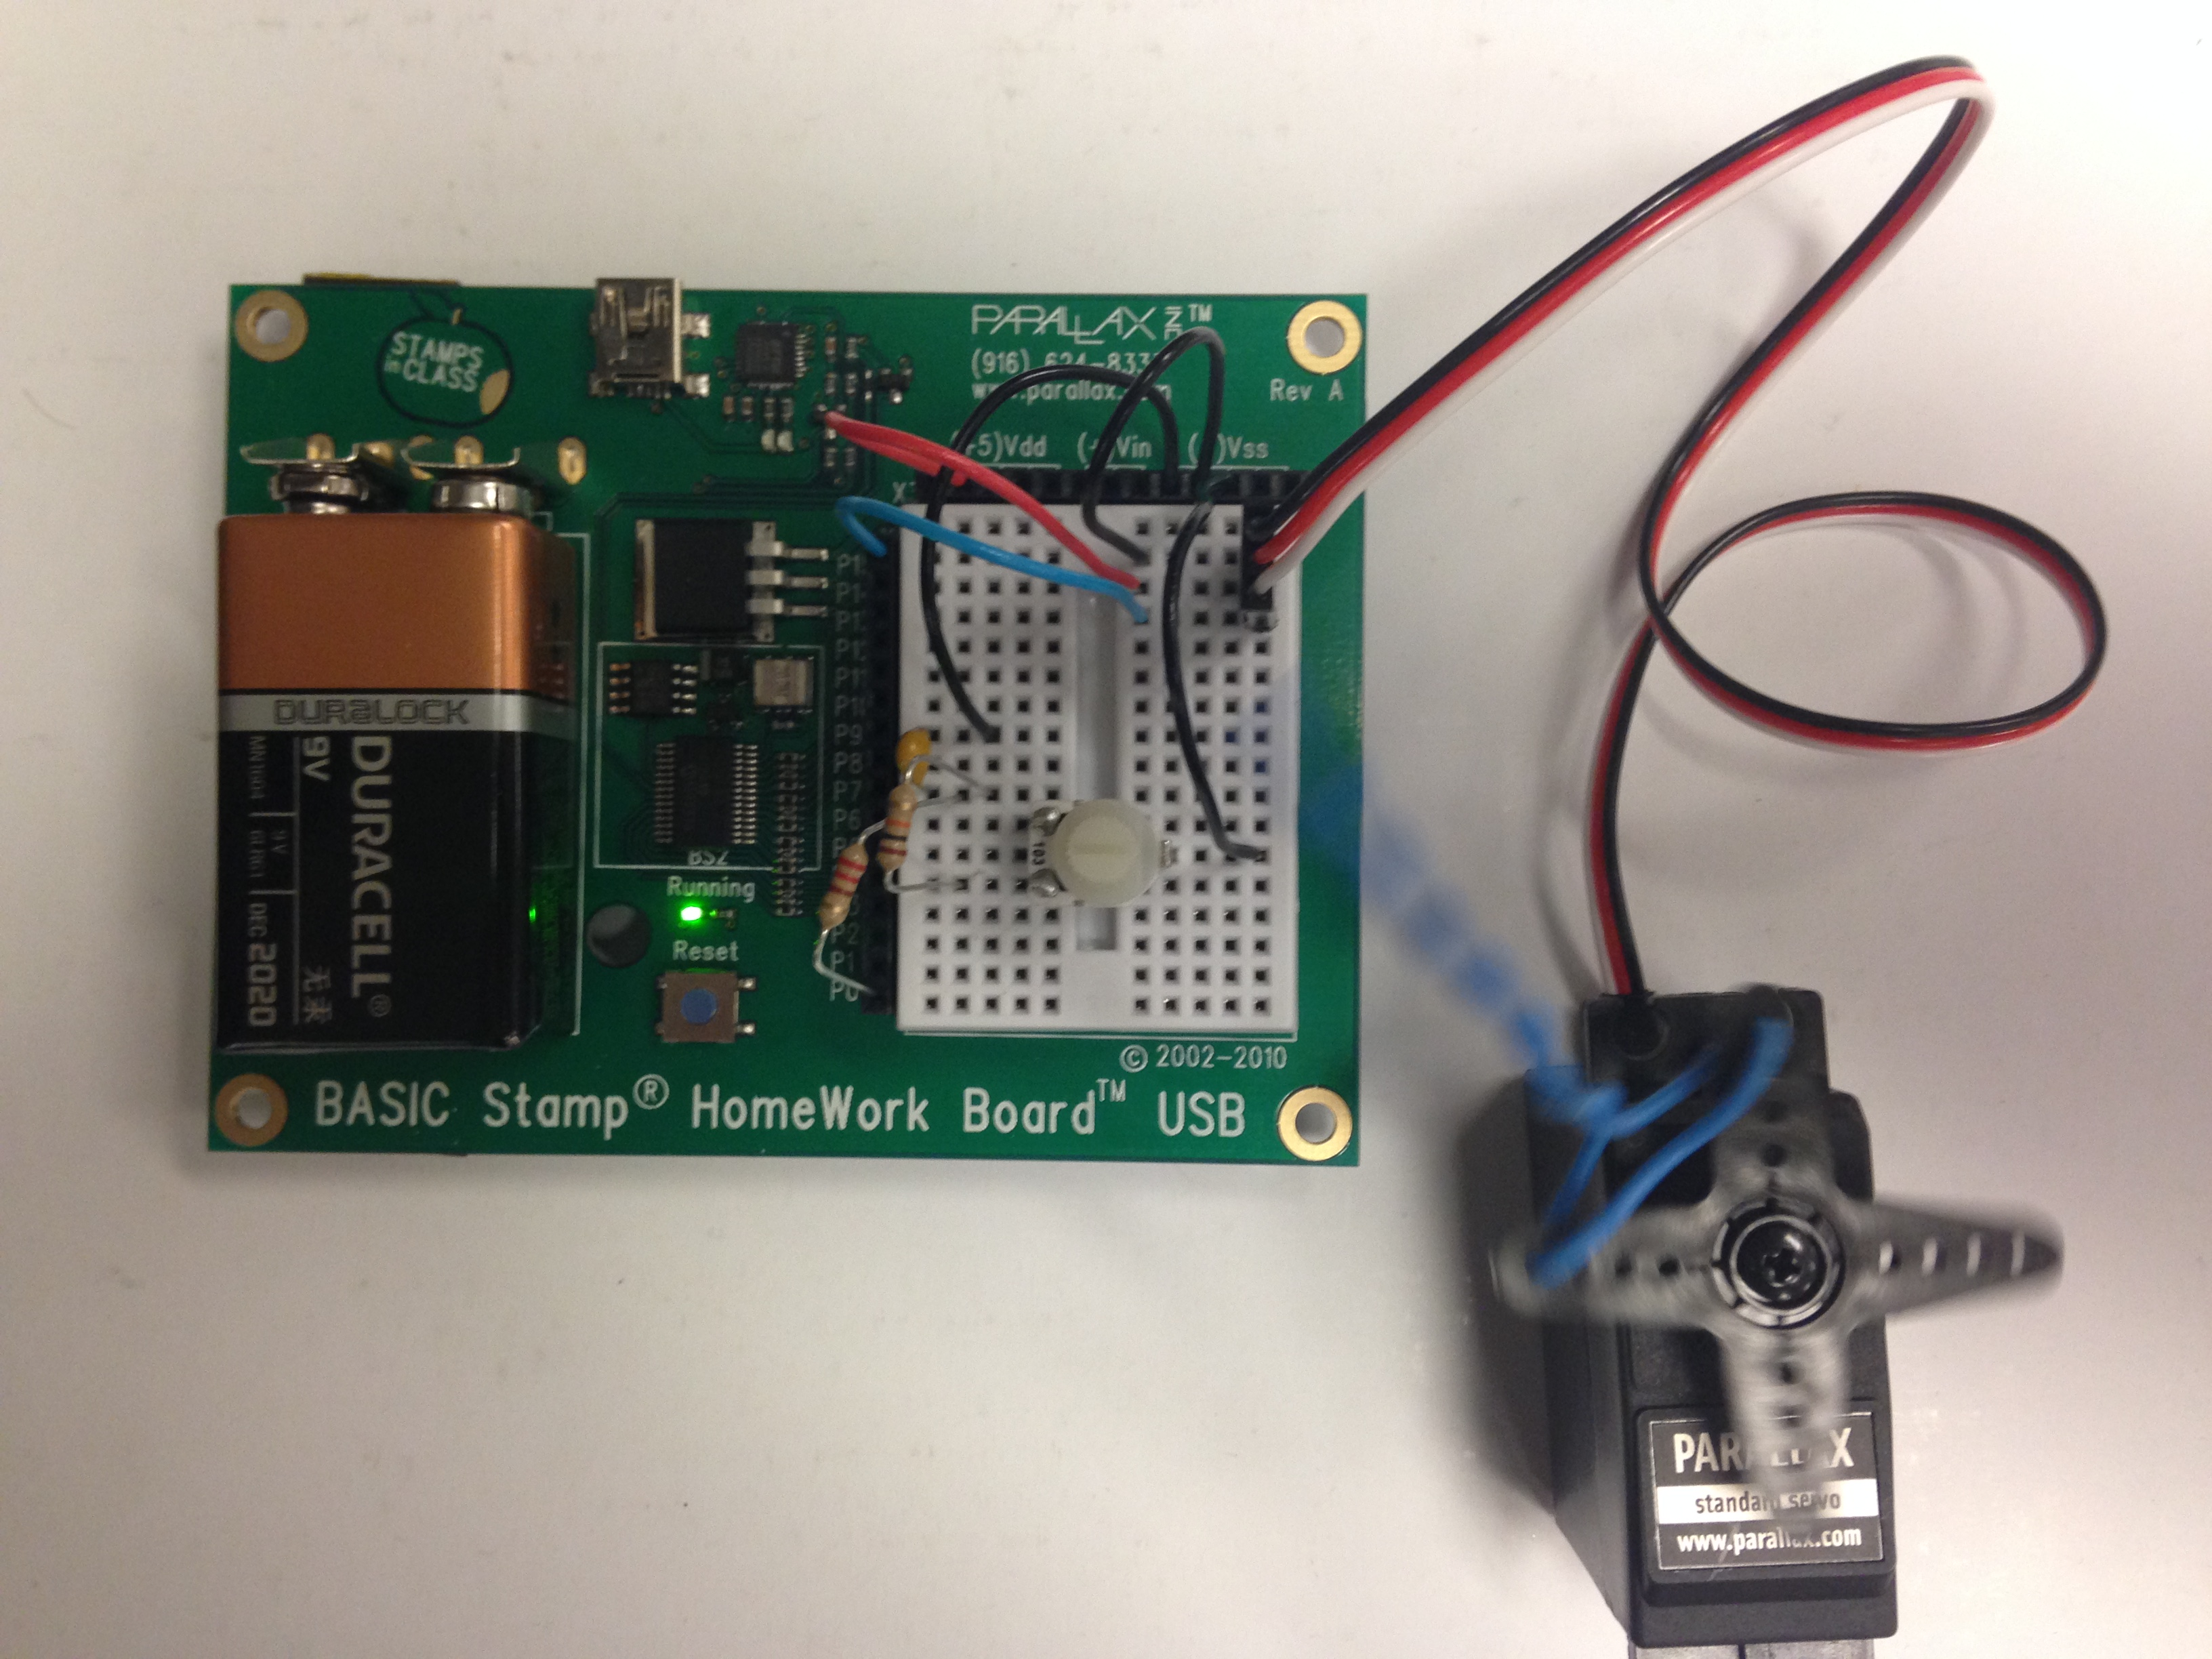
\includegraphics[width=0.6\textwidth]{wiper-controller.jpg}
\caption{Wiper Speed Controller Board}
\label{wiper-controller}
\end{figure}

\section{Discussion}

\section{Exercises}

There were no exercises given.

\clearpage
\section{Implementation Code}

\subsection{Rudder Controller}
\begingroup
\fontsize{11pt}{13pt}

\verbatiminput{Rudder-Controller.bs2}

\endgroup

\clearpage
\subsection{Wiper Controller}
\begingroup
\fontsize{9pt}{10pt}

\verbatiminput{Wiper-Controller.bs2}

\endgroup

\end{document}
